% --------------------------------------------------------------
% This is all preamble stuff that you don't have to worry about.
% Head down to where it says "Start here"
% --------------------------------------------------------------
 
\documentclass[12pt]{article}

\usepackage[margin=1in]{geometry} 
\usepackage{amsmath,amsthm,amssymb}
\usepackage[margin=1in]{geometry} 
\usepackage{amsmath,amsthm,amssymb}
%\usepackage[spanish]{babel} %Castellanización
\usepackage[T1]{fontenc} %escribe lo del teclado
\usepackage{inputenc} %Reconoce algunos símbolos
\usepackage{lmodern} %optimiza algunas fuentes
\usepackage{graphicx}
\graphicspath{ {images/} }
\usepackage{hyperref} % Uso de links

% To Display Chinese words
\usepackage{xeCJK}
% To Display Code
% \usepackage{listings}
\usepackage{minted}
% To Display csv file
\usepackage{csvsimple}
\usepackage{longtable}
\usepackage{booktabs}
 
\newcommand{\N}{\mathbb{N}}
\newcommand{\Z}{\mathbb{Z}}
 
\newenvironment{theorem}[2][Theorem]{\begin{trivlist}
\item[\hskip \labelsep {\bfseries #1}\hskip \labelsep {\bfseries #2.}]}{\end{trivlist}}
\newenvironment{lemma}[2][Lemma]{\begin{trivlist}
\item[\hskip \labelsep {\bfseries #1}\hskip \labelsep {\bfseries #2.}]}{\end{trivlist}}
\newenvironment{exercise}[2][Exercise]{\begin{trivlist}
\item[\hskip \labelsep {\bfseries #1}\hskip \labelsep {\bfseries #2.}]}{\end{trivlist}}
\newenvironment{problem}[2][Problem]{\begin{trivlist}
\item[\hskip \labelsep {\bfseries #1}\hskip \labelsep {\bfseries #2.}]}{\end{trivlist}}
\newenvironment{question}[2][Question]{\begin{trivlist}
\item[\hskip \labelsep {\bfseries #1}\hskip \labelsep {\bfseries #2.}]}{\end{trivlist}}
\newenvironment{corollary}[2][Corollary]{\begin{trivlist}
\item[\hskip \labelsep {\bfseries #1}\hskip \labelsep {\bfseries #2.}]}{\end{trivlist}}

\newenvironment{solution}{\begin{proof}[Solution]}{\end{proof}}

% write csv content in latex 
\begin{filecontents*}{grade.csv}
NUM, WIN RATE, END RATE
64,     100.0\ \%, 0.1\ \%
128,    99.9\ \%, 0.1\ \%
256,    99.8\ \%, 1.7\ \%
512,    98.1\ \%, 2.0\ \%
1024,   96.1\ \%, 4.7\ \%
2048,   91.4\ \%, 11.9\ \%
4096,   79.5\ \%, 77.7\ \%
8192,   1.8\ \%, 1.8\ \%
\end{filecontents*}
 
\begin{document}
 
% --------------------------------------------------------------
%                         Start here
% --------------------------------------------------------------
 
\title{2019 Deep Learning and Practice \\ Lab 7 -- Temporal Difference Learning}
\author{0756110 李東霖}

\maketitle
\section{Introduction}

Play 2048 through Temporal Difference Learning, a kind of Reinforcement Learning.

Requirements as follows:

\begin{itemize}
    \item Understand TD(0)
    \item Implement TD(0)
    \item Train 2048 agent with before-state and after-state
\end{itemize}

\subsection{Game Environment -- 2048}

There are UP, DOWN, LEFT, RIGHT four action in 2048 game. The reward of game is the value of new tile when two tiles are combined. For example, 4 and 4 can be combined as 8 and then the reward is 8.

\section{Experiment setup}

\subsection{Temporal Difference (0)}

Temporal Difference Learning is model-free algorithm thus it need estimate future reward by episodes of experience. But if like Monte-Carlo learns from complete episodes, its learning is slow. To avoid that problem, TD learns from incomplete episodes, also means learning from next few states. We can see equation of TD(0) as follow.

\begin{equation}
V(S_t) \leftarrow V(S_t) + \alpha (R_{t+1} + \gamma V(S_{t+1}) - V(S_t) )
\end{equation}

If $V(S_{t+1})$ is actual value, TD is unbias estimate. But $V(S_{t+1})$ is also from estimated. Therefore TD(0) is bias estimate. This is different from MC algorithm.

\subsection{Before state}

The game 2048 has a random state transition after doing action. 

\begin{equation}
    s_t \longrightarrow_{a_t} s_t' \longrightarrow_{random \ popup} s_t''
    , \  s_{t+1} = s_t''
\end{equation}

Before state means that estimate $s_t$ with $s_t''$. So use equation as follows:

\begin{equation}
    V(s_t) \leftarrow V(s_t) + \alpha (r + \gamma V(s_t'') - V(s_t))
\end{equation}

And find best action to use as follows:

\begin{equation}
    \arg \max \  r + \sum_{s' \in  P(s' | s, a), \  s'' \in P(s'' | s' )} P(s'' | s') V(s'')
\end{equation}

It means that find expectation of all possible $s''$ and choose maximum  expectation.

\subsection{After state}

Contrary to before state, after state estimate $s_t'$ with $s_{t+1}'$. So use equation as follows:

\begin{equation}
    V(s_t') \leftarrow V(s_t') + \alpha (r + \gamma V(s_{t+1}') - V(s_t'))
\end{equation}

And find best action to use as follows:

\begin{equation}
    \arg \max \  r + V(s_t')
\end{equation}

It means ignore random popup, only to estimate state after action.

\subsection{My implementation (python)}

\subsubsection{Game environment}

Game environment is reference from https://github.com/moporgic/2048-Demo-Python/. I added \verb|rotate|, \verb|end| and \verb|allpopup| functions. The \verb|rotate| function can rotate whole game board. The \verb|end| function can judge game is end or not. The \verb|allpopup| function can output all possible game after game pop up with probability.

\begin{minted}[frame=lines, breaklines]{python}
class board:
    """simple implementation of 2048 puzzle"""
    
    def __init__(self, tile = None, max_number=15):
        self.tile = tile if tile is not None else [0] * 16
        self.max_num = max_number
    
    def __str__(self):
        state = '+' + '-' * 24 + '+\n'
        for row in [self.tile[r:r + 4] for r in range(0, 16, 4)]:
            state += ('|' + ''.join('{0:6d}'.format((1 << t) & -2) for t in row) + '|\n')
        state += '+' + '-' * 24 + '+'
        return state
    
    def mirror(self):
        return board([self.tile[r + i] for r in range(0, 16, 4) for i in reversed(range(4))])
    
    def transpose(self):
        return board([self.tile[r + i] for i in range(4) for r in range(0, 16, 4)])
    
    def rotate(self):
        return board([self.tile[4*(3-(i%4)) + (i//4)] for i in range(16)])
    
    def left(self):
        move, score = [], 0
        for row in [self.tile[r:r+4] for r in range(0, 16, 4)]:
            row, buf = [], [t for t in row if t]
            while buf:
                if len(buf) >= 2 and buf[0] is buf[1]:
                    buf = buf[1:]
                    buf[0] += 1
                    score += 1 << buf[0]
                row += [buf[0]]
                buf = buf[1:]
            move += row + [0] * (4 - len(row))
        return board(move), score if move != self.tile else -1
    
    def right(self):
        move, score = self.mirror().left()
        return move.mirror(), score
    
    def up(self):
        move, score = self.transpose().left()
        return move.transpose(), score
    
    def down(self):
        move, score = self.transpose().right()
        return move.transpose(), score
    
    def popup(self):
        tile = self.tile[:]
        empty = [i for i, t in enumerate(tile) if not t]
        tile[random.choice(empty)] = random.choice([1] * 9 + [2])
        return board(tile)
    
    def allpopup(self):
        tile = self.tile[:]
        empty = [i for i, t in enumerate(tile) if not t]
        boards = []
        for i in empty:
            for n in [1] * 9 + [2]:
                tmp = tile.copy()
                tmp[i] = n
                boards.append(board(tmp))
        return boards
    
    def end(self):
        tile = self.tile[:]
        empty = [i for i, t in enumerate(tile) if not t]
        
        count_max_num = np.count_nonzero(self.max_num == np.array(tile))
        return len(empty) == 0 or count_max_num > 0
\end{minted}

\subsubsection{Tuple network}

I implemented a class to perform N-Tuple Network with all possible isomorphic pattern.

\begin{minted}[frame=lines, breaklines]{python}
def find_isomorphic_pattern(pattern):
    a = board(list(range(16)))

    isomorphic_pattern = []
    for i in range(8):
        if (i >= 4):
            b = board( a.mirror().tile )
        else:
            b = board( a.tile )
        for _ in range(i%4):
            b = b.rotate()
        isomorphic_pattern.append(np.array(b.tile)[pattern])
        
    return isomorphic_pattern

class TuplesNet():
    def __init__(self, pattern, maxnum):
        self.V = np.zeros(([maxnum]*len(pattern)))
        self.pattern = pattern
        self.isomorphic_pattern = find_isomorphic_pattern(self.pattern)
        
    def getState(self, tile):
        return [tuple(np.array(tile)[p]) for p in self.isomorphic_pattern]
    
    def getValue(self, tile):
        S = self.getState(tile)
        
        V = [self.V[s] for s in S]
        
        # sum all value from isomorphic pattern
        V = sum(V)

        return V
    
    def setValue(self, tile, v, reset=False):
        S = self.getState(tile)

        v /= len(self.isomorphic_pattern)
        V = 0.0
        for s in S:
            if not reset:
                # update value to isomorphic pattern
                self.V[s] += v
            else:
                # reset value to isonorphic pattern
                self.V[s] =  v
                
            V += self.V[s]
        return V
\end{minted}

\subsubsection{Agent}

First, create agent with specific patterns. The agent use patterns to create \verb|TuplesNet|.

\begin{minted}[frame=lines, breaklines]{python}
class Agent():
    def __init__(self, patterns, maxnum):
        self.Tuples = []
        for p in patterns:
            self.Tuples.append(TuplesNet(p, maxnum))
        self.metrics = []
        # if True, use after-state. Otherwise use before-state
        self.after = True
\end{minted}

Second, integrate agent with multiple \verb|TuplesNet| through \verb|getValue| and \verb|setValue|. That two function let agent store value based on state.

\begin{minted}[frame=lines, breaklines]{python}
    def getValue(self, tile):
        return sum([t.getValue(tile) for t in self.Tuples])
    
    def setValue(self, tile, v, reset=False):
        v /= len(self.Tuples)
        V = 0.0
        for t in self.Tuples:
            V += t.setValue(tile, v, reset)
        return V
\end{minted}

Third, implement \verb|evaluate| and \verb|learn|. I use \verb|self.after| to decide which method (before or after) to use. That two function let agent make decision through value function.

\begin{minted}[frame=lines, breaklines]{python}
    # get all s' and reward in next_games
    def evaluate(self, next_games):
        # TD(0)-after
        if self.after:    
            #  r + V(s')
            return [ng[1] + self.getValue(ng[0].tile) for ng in next_games]
        # TD(0)-before
        else:
            # r + \sum P(s''|s')V(s'')
            rs = []
            for ng in next_games:
                all_v = [ self.getValue(nng.tile) for nng in ng[0].allpopup() ]
                if len(all_v) == 0:
                    v = 0
                else:
                    v = sum(all_v) / len(all_v)
                rs.append(ng[1] + v)
            return rs
    
    def learn(self, records, lr):
        # learn from end to begin
        # records = [end .... begin]
        # (s, a, r, s', s'')
        
        # TD(0)-after
        if self.after:
            exact = 0.0
            for s, a, r, s_, s__ in records: 
                # V(s') = V(s') + \alpha ( r_next + V(s'_next) - V(s') )
                error = exact - self.getValue(s_)
                exact = r + self.setValue(s_, lr*error)
        # TD(0)-before
        else:
            #exact = self.getValue(records[0][4])
            exact = 0.0
            for s, a, r, s_, s__ in records:
                # V(s) = V(s) + \alpha (r + V(s'') - V(s))
                error = r + exact - self.getValue(s)
                exact = r + self.setValue(s, lr*error)
\end{minted}

Finally, I need a \verb|train| procedure to run TD(0) algorithm.

\begin{minted}[frame=lines, breaklines]{python}
    def train(self, epoch_size, lr=0.1, showsize=1000):
        start_epoch = len(self.metrics)
        for epoch in range(start_epoch, epoch_size):
            # init score and env (2048)
            score = 0.0
            game = board().popup().popup()
            records = []
            while True:
                # choose action
                next_games = [game.up(), game.down(), game.left(), game.right()]
                action = np.argmax(self.evaluate(next_games))
                
                # do action
                # s'
                next_game, reward = next_games[action]
                
                # save record (s, a, r, s')
                # records.insert(0, (game.tile, action, reward, next_game.tile) )
                
                # if game is same as before, end game
                if game.end():
                    break
                
                # s''
                next_game_after = next_game.popup()
                
                score += reward
                
                # save record (s, a, r, s', s'')
                records.insert(0, (game.tile, action, reward, next_game.tile, next_game_after.tile) )
                
                # s = s'' update state
                game = next_game_after
                
            #self.learn(records, lr / len(self.Tuples))
            self.learn(records, lr)
            
            # store score, game len, end game board
            self.metrics.append( (score, len(records), game.tile) )
            if (epoch+1) % showsize == 0:
                clear_output(wait=True)
                self.showStattistic(epoch+1, showsize)
\end{minted}

And also implement some utility function to make convenient.

\begin{minted}[frame=lines, breaklines]{python}
    def showStattistic(self, epoch, unit, show=True):
        metrics = np.array(self.metrics[epoch-unit:epoch])
        
        # get average score
        score_mean = np.mean(metrics[:, 0])
        # get max score
        score_max = np.max(metrics[:, 0])
        
        if show:
            print('{:<8d}mean = {:<8.0f} max = {:<8.0f}'.format(epoch, score_mean, score_max))
        
        if (metrics.shape[1] < 3):
            return score_mean, score_max
        
        # all end game board
        end_games = metrics[:, 2]
        
        reach_nums = np.array([1<<max(end) & -2 for end in end_games])
                  
        if show:
            print('\n')
        
        score_stat = []
        
        for num in np.sort(np.unique(reach_nums)):
            # count how many game over this num
            reachs = np.count_nonzero(reach_nums >= num)
            reachs = (reachs*100)/len(metrics)
            
            # count how many game end at this num
            ends = np.count_nonzero(reach_nums == num)
            ends = (ends*100)/len(metrics)
            
            if show:
                print('{:<5d}  {:3.1f} % ({:3.1f} %)'.format(num, reachs, ends) )
            
            score_stat.append( (num, reachs, ends) )
        
        score_stat = np.array(score_stat)
        
        return score_mean, score_max, score_stat
    
    # use current state of game, return next game and action
    def play(self, game):
        next_games = [game.up(), game.down(), game.left(), game.right()]
        action = np.argmax(self.evaluate(next_games))
                
        next_game, reward = next_games[action]
        return next_game, reward, ['up', 'down', 'left', 'right'][action]
\end{minted}

\subsubsection{Main}

\begin{minted}[frame=lines, breaklines]{python}
MAX_NUM = 15 # 1<<15 == 32768
PATTERNS = [
    [0,1,2,3,4,5],
    [4,5,6,7,8,9],
    [0,1,2,4,5,6],
    [4,5,6,8,9,10]
]
random.seed(756110)
agent = Agent(PATTERNS, MAX_NUM)
agent.train(100000)

showCurve(agent.metrics, size=1000)
showWinRate(agent.metrics, [1024, 2048, 4096])
\end{minted}

\section{Experimental results}

\subsection{Score curves in Training}

\begin{figure}[H]
\centering
% \includegraphics[width=\linewidth]{path/to/image}
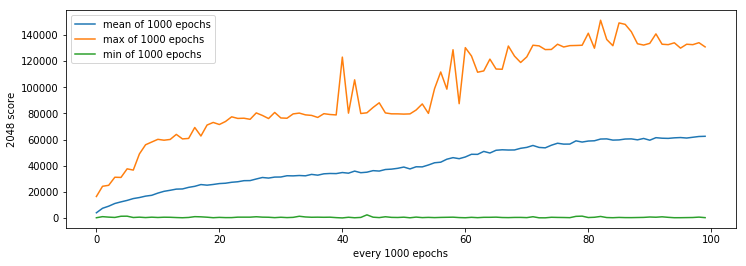
\includegraphics[width=\linewidth]{Images/scorecurve.png}
\caption{max/min/mean score curves every 1000 epoch}
\end{figure}

\subsection{Win rate curves in Training}

\begin{figure}[H]
\centering
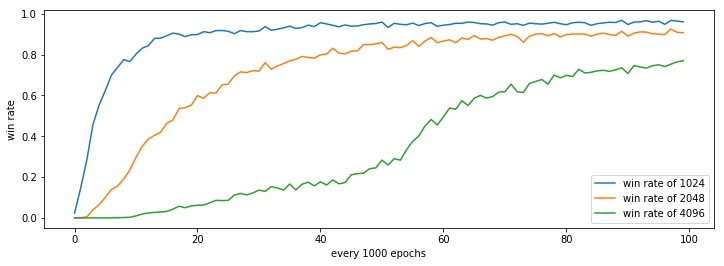
\includegraphics[width=\linewidth]{Images/winratecurve.png} 
\caption{1024 2048 4096 win rate curve every 1000 epoch}
\end{figure}

\subsection{Agent performance}

I use this agent to play 2048 with 1000 times.

\begin{table}[H]
    \centering
    \csvautobooktabular{grade.csv}
    \caption{agent performance}
    \label{tab:my_label}
\end{table}

The \verb|NUM| columns means which number on 2048 tile. The \verb|WIN RATE| columns means how many game can reach number on tile. The \verb|END RATE| columns means how many max of number on tile at end game.

\section{Discussion}

\subsection{Before state v.s. After state}

My before state is very bad than after state. I think before state need all possible $s''$. But all $s''$ usually are wrong value in the begin. And number of state is huge. The before state has slow learning because of that reason.

\begin{figure}[H]
\centering
% \includegraphics[width=\linewidth]{path/to/image}
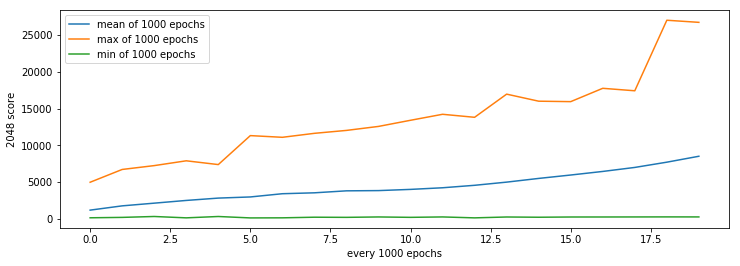
\includegraphics[width=\linewidth]{Images/beforescorecurve.png}
\caption{ [Before state] max/min/mean score curves every 1000 epoch}
\end{figure}

% --------------------------------------------------------------
%     You don't have to mess with anything below this line.
% --------------------------------------------------------------
 
\end{document}